
\lohead{Vollmaier Alois}

\chapter{Informatik}\label{ch:informatik}


%@COPYRIGHT VOLLMAIER ALOIS
\section{Zeitplan}\label{subsec:zeitplan}

\begin{figure}[]
    \begin{center}
\scalebox{0.6}{
        \begin{ganttchart}[
        hgrid style/.style={black, dotted},
        calendar week text={\currentweek},
        vgrid={*6{white, dotted}, *1{black, dashed}},
        x unit=1mm,
        group label font=\bfseries \Large,
        y unit chart=9mm,
        y unit title=12mm,
        time slot format=isodate,
        time slot unit=year
        link/.style={->, thick}
        ]{2019-09-2}{2020-03-15}
            \gantttitlecalendar{year, month=name, week}\\

            \ganttgroup[
            group/.append style={fill=red}
            ]{Backend-Programmierung}{2019-09-02}{2019-11-15}\\ [grid]
            \ganttbar[
            bar/.append style={pattern=north east lines},
            name=Konzeptplanung
            ]{Konzeptplanung}{2019-09-02}{2019-09-25}\\ [grid]
            \ganttbar[
            bar/.append style={pattern=north east lines},
            name=Einrichtung - Arbeitsumgebung
            ]{Einrichtung - Arbeitsumgebung}{2019-09-15}{2019-10-1}\\ [grid]
            \ganttbar[
            bar/.append style={pattern=north east lines},
            name=Start-Programmierung
            ]{Programmierung}{2019-10-05}{2019-11-15}

            \ganttnewline[thick, black]

            \ganttgroup[
            group/.append style={fill=blue}
            ]{Frontend-Programmierung}{2019-11-15}{2019-12-22}\\ [grid]
            \ganttbar[
            bar/.append style={pattern=north east lines},
            name=Konzeptplanung
            ]{Konzeptplanung}{2019-11-15}{2019-11-31}\\ [grid]

            \ganttbar[
            bar/.append style={pattern=north east lines},
            name=Start-Programmierung
            ]{Programmierung}{2019-11-31}{2019-12-22}

            \ganttnewline[thick, black]

            \ganttgroup[
            group/.append style={fill=green}
            ]{Testen - Aufbauen}{2019-12-22}{2020-02-01}\\ [grid]


            \ganttlink[link mid=0.75]{Konzeptplanung}{Start-Programmierung}
            \ganttlink{Einrichtung - Arbeitsumgebung}{Start-Programmierung}
        \end{ganttchart}
}
    \end{center}
    \caption{Zeitplanung - Informatik}
\end{figure}

%@COPYRIGHT VOLLMAIER ALOIS

\section{Anforderungen und Ziele}\label{subsec:anforderungen-und-ziele}

\subsection{Fronted-Programmierung}
\subsection{Backend-Programmierung}
\subsection{Hardwarenahe-Programmierung}

Im Allgemeinen besteht das Ziel darin, eine für Benutzer freundliche GUI, zu bauen, welche schlussendlich im Betrieb der Maschiene auf einem 7" Display angezeigt wird. Auf dieser Grafischen Oberfläche soll es Möglich sein, die Steuerung der Maschiene zu übernehmen.
Dies bedeutet im engsten Sinne, dass Befehle zwischen den 2 Systemen, also dem Rasperry PI 3B+ und der Ansteuerplatine ausgetauscht werden müssen.\\\\
Die Möglichkeiten des Benutzers, die Maschiene zu bedienen sollen folgende Kernpunkte beinhalten:
\begin{enumerate}
    \item Ausgabe von einzelnen Spielkarten
    \item Konfigurierung von Spielmodi, welche Einstellungen zum Spiel beinhalten
    \item Das Zählen von Punkten und dessen Visualisierung am Display
    \item Ausschalten der Maschiene
    \item Übersicht aller vergangenen Spiele
\end{enumerate}
Ziel ist es dieses Interface so übersichtlich wie möglich zu gestalten. Dies soll durch unterschiedliche Tabs realisiert werden.\\\\
Zusätzlich soll im Hintergrund eine sogenannte Log-Datei automatisch vom Programm geschrieben werden. Diese bringt dem Entwicker einen enormen Mehrwert im Bereich des Fehler-Handlings. \\
Um etwaiige Einstellungen der Seriellen Schnittstelle sowie die definition der Pfade für Log-Dateien außerhalb des Programmes vorzunehmen, ist es auch nötig, eine Konfigurationsdatei zu erstellen, welche nach jedem Start vom Programm eingelesen wird. Mit dieser Config-Datei wird auch die Möglichkeit geschafffen,
Spielmodi zu speichern und zu verändern.

Die Speicherung der vergangenen Spiele soll außerdem auch in einer eigenen Datei vonstatten gehen. Name des ausgewählten Spielmoduses, dessen Hintergrundinformationen, Spielernamen und Punkteanzahl sollen die Kernstücke jedes Eintrags in die Datei sein.\newpage

\subsection{Voruntersuchung}\label{subsec:voruntersuchung}

\subsubsection{Auswahl des GUI-Toolkits}
Die Auswahl des für die Anwendung am besten geeigneten GUI-Toolkits, spielt eine wesentliche Rolle in der programmierung von grafischen Anwendungen. Diese Toolkits stellen meist alle Elemte zur Erstellung einer GUI bereit. Diese sind z.B. Knöpfe, Listen und Textfelder mit denen der Benutzer ineragieren kann.

\textbf{Swing}
Das bereits in der Standart Java Bibliothek verfügbare Java Swing bietet die Möglichkeit komplexe Oberflächen zu erstellen. Der Aufwand zur Einrichtung hält sich in Grenzen denn im Vergleich zu Java-FX muss hier nicht extern in einem eigenen Programm gearbeitet werden, um die GUI zu erstellen.
Aufgrund der Verfügbarkeit von Java Swing in der Java Bibliothek bieten alle IDE's die Möglichkeit zur erstellung von Oberflächen. Das etwas veraltete und lieblose Look and Feel von Java Swing brachte uns zur Entscheidung, den Nachfolger, nähmlich Java FX, zu verwenden.

\textbf{JavaFX}
Der Nachfolger von Java Swing ist Java FX. Hierbei werden im Vergleich zu Java Swing nicht alle GUI Elemente in einer Datei beschrieben, was die Übersichtlichkeit beeinträchtigt, sondern die Beschreibung geschieht in externen FXML-Dateien.
Die Basis dieser FXML-Dateien ist XML, eine Sprache zur Darstellung von Daten in einem von Menschen lesbaren Format. Der Code hinter der GUI befindet sich jedoch nicht in diesen Dateien sondern in eigenen Controller Klassen, welche mit der GUI verknüpft sind. Dies bringt enorme Vorteile mit sich, denn die strikte Trennung zwischen Beschreibenden Elementen der GUI
und dem dahinter stehenden Code ist dadurch möglich.\\
Auch bieter Java FX die Möglichkeit, seperate Stylesheets, also Dokumente, in welchen das Aussehen von Elementen beschrieben wird, zu erstellen.


\subsubsection{Auswahl der IDE}
Bevor mit dem Programmierprozess gestartet werden kann, ist es notwendig, eine für IDE auszuwählen, welche alle Anforderungen erfüllt. In unserem Fall sind diese im Speziellen:
\begin{enumerate}
    \item Möglichkeiten der Remote-Programmierung sowie dem Debuggen
    \item Einfacher Workflow
\end{enumerate}

\textbf{Netbeans IDE}
Die Netbeans IDE ist eine Open-Source Entwicklungsumgebung, welche selbst in der Programmiersprache Java geschrieben wurde und damit plattformunabhängig ist. Primär wurde sie Entwickelt, um Programme in der Programmiersprache Java zu erstellen.\\
Große Vorteile bringt diese IDE im Bereich der Remote-Programmierung mit sich. Die Möglichkeit, eine Remote-Plattform einzurichten wurde einfach gelöst und das Arbeiten verläuft meist ohne Probleme.
Realisierung
\textbf{Intellij IDE}
Eine kostenpflichtige Alternative zu Netbeans ist Intellij. Aufgrund der komplizierten Einrichtung eines Remote-Systems, sowie dessen Handhabung im täglichen Arbeitsprozess wurde deutlich, dass Netbeans im wichtigsten Kriterium besser abschneidet. Darum fiel unsere Wahl auch auf diese IDE.

\subsubsection{Fragestellung zur Verwendung eines Build-Tools}
\section{Backend-Programmierung}
\subsection{Entwurdsmuster Singelton}
\subsection{Kommunikation - serielle Schnittstelle}
\subsubsection{Konzept}

Um erfolgreich Daten zwischen dem Raspberry PI 3B+ und der Platine, welche die Ansteuerung sämtlicher Komponenten übernimmt, zu übertragen, wird ein Kommunikationsprotokoll benötigt.
Dieses Protokoll stellt im engsten Sinne eine Vereinbarung dar, wie die Datenübertragung zwischen zwei oder mehreren Parteien abläuft. Anforderungen an dieses Protokoll sollen sein:
\begin{enumerate}
    \item einfache Integration in die Zielsysteme
    \item erweiterbarkeit des Protokolls mit geringem Arbeitsaufwand
    \item hohe Sicherheit gegenüber Übertragungsfehler
    \item schnelle Fehlererkennung sowie Fehlerbehebung
\end{enumerate}
Neben standartisierten Protokollen wie Modbus, Feldbus oder CAN-Bus gibt es die Möglichkeit selbst ein sogenanntes propretäres Übertragungsprotokoll zu kreieren. Dies ist in unserem Fall nötig, um alle Anforderungen abzudecken.
Basierend auf dem Master - Slave Prinzip, wobei der Rasperry PI den Master und die Ansteuerplatine den Slave darstellt, soll ein abgewandeltes Modbus ASCII Protokoll umgesetzt werden.

Zusätzlich soll, um die Anforderung des einfachen Fehlerhandlings zu erfüllen, ein Simulator ausprogrammiert werden, welcher auf Softwarebebene den Platz des Slaves bzw. der Ansteuerplatine einnimmt.
Der Startvorgang des Simulators soll mit einer einfachen modifizierung der Konfigurationsdatei vonstatten gehen.

\begin{figure}[H]
    \centering
    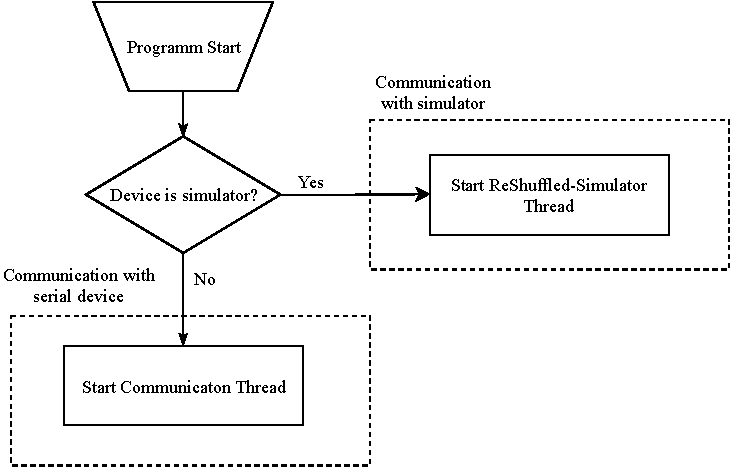
\includegraphics[width=0.8\textwidth]{fig/ainf/DeviceSelection}
    \caption{Schematische Darstellung der Geräteauswahl}
\end{figure}
\subsubsection{Übertragungsprotokoll}
\begin{table}[h]
    \centering
    \begin{tabular}{|
    >{\columncolor[HTML]{FFFFFF}}l |
    >{\columncolor[HTML]{FFFFFF}}l |
    >{\columncolor[HTML]{FFFFFF}}l |
    >{\columncolor[HTML]{FFFFFF}}l |
    >{\columncolor[HTML]{FFFFFF}}l |}
        \hline
        \textbf{Doppelpunkt :} & \textbf{Daten (ASCII)} & \textbf{Trennzeichen \#} & \textbf{CRC32-Prüfsumme} & \textbf{Semicolon \textbackslash{}n} \\ \hline
        8-Bit & 16-Bit & 8-Bit & 32-Bit & 8-Bit                                \\ \hline
    \end{tabular}
    \caption{Visualisierung des Datenakets}
\end{table}

Das verbindugslose ProtokollRealisierung ist wie in der Konzeptbeschreibung Master-Slave orientiert. Die Datenübertragung erfolgt textuell wobei nur Großbuchstaben verwendet werden dürfen.\newline\newline
Wie aus der oben dargestellten Tabelle zu entnehmen, ist der Aufbau eines Frames klar definiert. Der eindeutige Start des Datenpakets, welcher mit einem Doppelpunkt (:) eingeleitet wird, sowie das ebenfalls eindeutige Ende, umgesetzt mit einem Line Feed Character (),
bringt eindeutige Vorteile mit sich. Im Gegensatz zu anderen Protokollen wie z.B. Modbus RTU, muss hier nicht auf das Ende des Pakets "gewartet" werden. Dies führ oft zu Einbußen im Bereich der Performance und ist für uns nicht zielführend.\newline\newline
Gefolgt von dem Startzeichen folgen nun die Daten. Diese beinhalten eindeutig definierte Zecichenfolgen, welche verwendet werden um verschiedenste Zustände der Ansteuerplatine auszuführen. Diese Um auch hier zu wissen, wo sich das der Nutzdaten befindet, schließt das Trennzeichen () diese ab.\newline\newline
Um nun die Integrität, also die Korrektheit der Daten bei einer Übertragung zu überprüfen, wird im nächsten Schritt eine Prüfsumme verwendet. Ziel dieser ist es, anhand der Nutzdaten einen Wert zu bilden, welcher danach vom Sender im Frame gespeichert bzw übertragen wird.
Der Empfänger berechnet nun mit dem selben Verfahren die Prüfsumme aus den empfangenen Daten und vergleicht diese mit der Übertragenen Prüfsumme des Senders. Sind beide Prüfsummen identisch, war die Übertragung erfolgreich und die Daten sind mit großer Wahrscheinlichkeit korrekt.
Stimmen diese nicht überein liegt ein Fehler vor. Die wichtigsten Arten von Übertragungsfehlern sind:
\begin{enumerate}
    \item Einzelbitfehler (1 Bit verändert)
    \item Burstfehler (ganze Folge von Bits verändert)
\end{enumerate}

Neben einfachen Verfahren wie z.B. dem Paritätsbit-Verfahren gibt es auch Komplexere. Die zyklische Redundanzprüfung, auch CRC genannt, ist eines davon. Sie ist realtiv einfach zu realisieren und dennoch wirkungsvoll.
Wichtig beim CRC-Verfahren ist, dass beide Teilnehmen, also Sender und Empfänger, das selbe Generator-Polynom verwenden. Der Grad des Generatorpolyoms beträgt in unserem Fall 32 (CRC-32).

\subsubsection{Entwurdsmuster Command}
\subsubsection{Request- und Responsehandling}

\subsection{Kommunikation - Debugging-Simulator}
\subsubsection{Konzept und Gründe zur Erstellung}
\subsubsection{Datenaustausch}
\subsubsection{Verarbeitung ankommender Daten}


\subsection{Logging}
\subsubsection{Grundlagen}
\subsubsection{Integration in das Programm}
\subsection{Konfiguration}
\subsubsection{Grundlagen zu Gson}
\subsubsection{Datenmodelle}
\subsubsection{Verwahrung am Zielsystem}

\subsection{Statistiken}
\subsubsection{Konzept}
\subsubsection{Datenmodelle}
\subsubsection{Verwahrung am Zielsystem}

\subsection{Controllerklassen}
\subsubsection{Grundlagen}
\subsubsection{StartupController}
\subsubsection{MainController}
\subsubsection{HomeController}
\subsubsection{StatsController}
\subsubsection{About- und HelpController}


\section{Frontend-Programmierung}
\subsection{Designkonzept}
\subsection{Entwurfsmuster MVC}
\subsubsection{Grundlagen}
Das MVC-Design Pattern, auch Model-View-Controller Design Pattern ist eines der weit verbreiteste Design Patterns. Es dient zur Strukturierung von Anwendungen und teilt diese in 3 große Bereiche ab, welche strikt von einander getrennt sind.
Mithilfe dieser Strukturierung fällt es dem Programmierer wesentlich leichter, spätere Änderungen bzw. Erweiterungen am Projekt durchzuführen. Auch ist es nun möglich pararell an dem Programm zu arbeiten den Ersteller von GUI und Ersteller des Controllers, also der Berechnungen dahinter, sind nun nicht mehr voneinander Abhängig.
\newpage
\begin{wrapfigure}{r}{0.5\textwidth}
    \vspace{-310pt}
    \begin{center}
        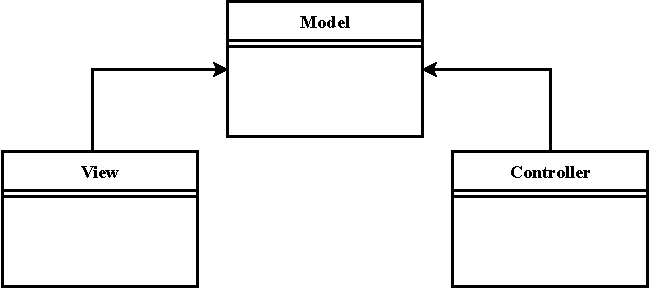
\includegraphics[width=0.17\textwidth]{fig/ainf/ModelViewController.pdf}
    \end{center}
    \caption{MVC-Design Pattern}
    \vspace{20pt}
\end{wrapfigure}


\begin{enumerate}
    \item \textbf{View}  \\
    Datenrepräsentation\\
    Organisiert alle Kontrollelemente
    \item \textbf{Controller} \\
    Stellt die Verbindung zwischen View und Model her\\
    Verwaltet Benutzerinteraktion und enthält Steuerlogik
    \item \textbf{Model} \\
    Datenrepräsentation\\
    Ist von der Benutzerschnittstelle komplett abgeschirmt
\end{enumerate}
\vspace{20pt}

\subsubsection{Integration anhand eines Programms}
Um zu zeigen, wie das MVC-Pattern in der Realität umgesetzt wird, ist im folgenden ein Beispiel dargestellt. Ziel des Programms ist es, einen Wert mithilfe eines Buttons hochzuzählen und auf einem Label im View anzeigen zu lassen.
Sobald der Knopf "Increment by 1" betätigt wird, soll der Wert um 1 erhöht werden.
\begin{lstlisting}[style=java,caption=Java Codebeispiel,label=Hauptprogramm]
    public class Main extends Application {
    @Override
    public void start(Stage stage) throws Exception {
    Model model = new Model();
    View view = new View(model, stage);
    Controller controller = new Controller(model, view);
    }
    public static void main(String[] args) {
    launch(args);
    }
    }
\end{lstlisting}


\begin{lstlisting}[style=java,caption=Java Codebeispiel,label=Model]
public class Model extends Observable{
private int counter;
public Model() {
}
public int getCounter() {
return countDown;
}
public void increment() {
if (counter > 0) {
counter++;
}
notifyObservers();
}
\end{lstlisting}

\begin{lstlisting}[style=java,caption=Die Klasse View,label=View]
public class View implements Observer {
private Model model;
private Stage stage;
private Label label;
private Button countButton;
public View(Model model, Stage stage) {
this.model = model;
this.stage = stage;
label = new Label("Counter: " + model.getCounter());
btIncrement = new Button("Increment by 1");
stage.setScene(new Scene(new VBox(label, countButton)));
model.addObserver(this);
}
@Override
public void update(Observable o, Object arg) {
label.setText("Counter: " + model.getCounter());
\end{lstlisting}



\subsection{Beschreibung der View-Elemente}
\subsubsection{Grundlagen zu SceneBuilder}
\subsubsection{Verwendung von Material Design Bibliotheken}

\subsection{Utility Klassen zur GUI}
\subsubsection{AlertUtil}
\subsubsection{GuiUtil}


\subsection{Implementierung von CSS}
\subsubsection{StartupCSS}
\subsubsection{HomeCSS}
\subsection{Internationalisierung}
\subsubsection{Gründe der Umsetzung}
\subsubsection{Integration in das Interface}
\subsubsection{Ressourcen Manager}
\subsubsection{Resource Utility}
\subsubsection{Bereitgestellte Ressources Bundles}

\section{Hardwarenahe-Programmierung}
\subsection{Einrichtung des Mikrocontrollers}
\subsection{Konzept und Ablaufdiagramm zur Kartenausgabe}
\subsection{Request- und Responsehandling}
\section{Teilaufbau}
\subsection{Auswahl des Zielsystems}
\subsubsection{Arduino}
\subsubsection{Raspberry PI}
\subsection{Auswahl des Displays}
\subsection{Montage und Testaufbau}
\subsection{Konfiguration des Zielsytsems}
\subsubsection{Betriebssystem}
\subsubsection{Speichermedium}
\subsubsection{Touchpanel}
\subsubsection{SSH und SFTP}
\subsubsection{Autostart realisiert durch Services}

\section{Probleme - Verbesserungsmöglichkeiten - Zusammenfassung}
\subsection{Probleme}
\subsubsection{Probleme bei der Implementierung von JavaFX}
\subsubsection{Kommunikation zwischen Controllern}
\subsubsection{}
\subsection{Verbesserungsmöglichkeiten}
\subsubsection{Online Update-Möglichkeit der Software}
\subsubsection{Smartphone-Interface zum Zählen der Punkte}
\subsection{Zusammenfassung}